\chapter{Traffic Control}
Traffic control in Linux is realized using a tool named \acs{TC}. It consists of four basic techniques.

\begin{enumerate}
\item \textbf{Shaping}: This is the technique we will be using in order to enforce an upper bandwidth limit. But in general, it is the process of manipulating the bandwidth. It can also be used to smooth out bursts in order to improve the quality of service. Shaping is done on egress traffic.

\item \textbf{Scheduling}: This is the process of staging packets according to a schedule. Like this reordering of packets can be achieved. Scheduling as well happens with egress traffic.

\item \textbf{Policing}: This is the equivalent to shaping but for ingress traffic. It is worth noticing that traffic policing is more limited than traffic shaping, since there is no ingress queue.

\item \textbf{Dropping}: This is a quite primitive approach of just dropping traffic that exceeds a given bandwidth. This is applicable for both ingress and egress traffic.
\end{enumerate}

For our needs, traffic shaping fits best. But since we need to limit ingress traffic as well, and shaping only operates on egress traffic, we need a workaround. More about that in section  \ref{Ingress Traffic}. Traffic control using \acs{TC} is implemented using tree basic building blocks: \acp{QDISC}, classes and filters. They will be discussed in section \ref{TC}.

\section{Theory}
\subsection{Traffic Shaping}
As previously stated, traffic shaping happens with egress traffic. However, there is a special \acs{QDISC} that is handling ingress traffic. Since this \acs{QDISC} is the only one applicable on ingress traffic, it is called \textit{ingress}. The term \acl{QDISC}, in that case, is a bit misleading, because there is no such thing as an ingress queue. All the other \acsp{QDISC} handle egress traffic and are quite diverse. Each \acs{QDISC} has a shaping algorithm that shapes the traffic passing the corresponding \acs{QDISC}. \acsp{QDISC} can be either classful or classless (such as the ingress \acs{QDISC}). Classful \acsp{QDISC} have a shaping algorithm that can handle traffic, which is classified in different classes, differently. Both the classes and the classifiers, which are filters that determine which kind of traffic belongs to which class, are attached to the \acs{QDISC}. Classless \acsp{QDISC} can obviously not handle classes. However they can handle filters, which can either do policing on the traffic or i.e. redirect it to a different interface.
\subsection{Egress Traffic}

\subsection{Ingress Traffic} \label{Ingress Traffic}
\subsubsection{Traffic Policing using Filters}
\subsubsection{Traffic Shaping using Virtual Interfaces}
\begin{figure}[h]
	\centering
	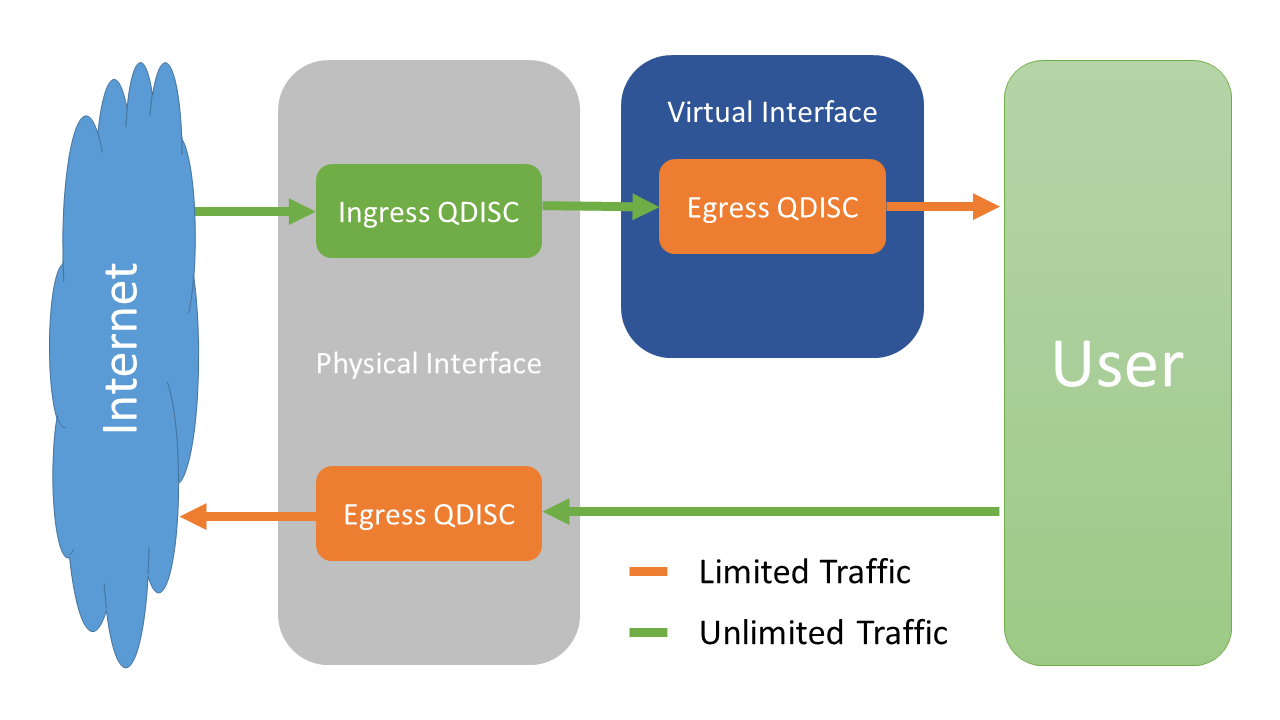
\includegraphics[width=\textwidth]{img/Interface-Setup.png}
	\caption{Interface set-up}
	\label{Interface set-up}
\end{figure}
\section{TC} \label{TC}
\subsection{Queuing Disciplines}
\subsection{Classes}
\subsection{Filters}